\documentclass[11pt,a4paper]{article}

\usepackage[T1]{fontenc}
\usepackage[utf8]{inputenc}
\usepackage{lmodern}
\usepackage[margin=2.2cm]{geometry}
\usepackage{microtype}
\usepackage{booktabs}
\usepackage{tabularx}
\usepackage{array}
\usepackage{enumitem}
\usepackage{xcolor}
\usepackage{amssymb}
\usepackage{caption}
\usepackage[section]{placeins}
\usepackage{tikz}
\usetikzlibrary{positioning,arrows.meta,decorations.pathmorphing,calc,shapes.geometric,fit,backgrounds}
\usepackage[hidelinks]{hyperref}
\usepackage[capitalise,nameinlink,noabbrev]{cleveref}

\hypersetup{
  pdftitle={Scenario and System Model},
  pdfauthor={Aditya Sissodiya},
  pdfsubject={Command succession in an intermittently connected incident journal: for sign-off},
}
\pdfinfoomitdate=1
\pdftrailerid{}

% Colours shared with the meeting slides.
\definecolor{ink}{HTML}{1F2A44}
\definecolor{accent}{HTML}{2F6DB5}
\definecolor{good}{HTML}{2E7D32}
\definecolor{warn}{HTML}{C0392B}
\definecolor{resid}{HTML}{E08E0B}
\definecolor{doubt}{HTML}{7B1FA2}
\definecolor{prov}{HTML}{8A94A6}
\definecolor{soft}{HTML}{EEF2F8}

\setlist{leftmargin=*,topsep=3pt,itemsep=2pt}
\renewcommand{\arraystretch}{1.25}
\newcolumntype{L}{>{\raggedright\arraybackslash}X}
\newcolumntype{P}[1]{>{\raggedright\arraybackslash}p{#1}}
\captionsetup{font=small,labelfont=bf}
\setlength{\parskip}{4pt}
\setlength{\parindent}{0pt}

\newcommand{\status}[2]{\textcolor{#1}{$\bullet$}\,\textit{#2}}
\newcommand{\sAuth}{\status{good}{authoritative}}
\newcommand{\sProv}{\status{prov}{provisional}}
\newcommand{\sResid}{\status{resid}{residual}}
\newcommand{\sDoubt}{\status{doubt}{in doubt}}
\newcommand{\tick}{$\square$\ }

\title{\textbf{Scenario and System Model}\\[4pt]
\large Command succession in an intermittently connected incident journal}
\author{Aditya Sissodiya}
\date{}

\begin{document}
\maketitle
\thispagestyle{empty}

\noindent\colorbox{soft}{\parbox{\dimexpr\linewidth-2\fboxsep\relax}{\vspace{3pt}%
\textbf{What I ask of you.} Read this once, then sign it off or mark what should change.
It fixes the scenario (\S\S\ref{sec:incident}--\ref{sec:journal}), the line between what
the organization decides and what the system does (\S\ref{sec:split}), the translation
from org chart to system with our answer on consensus (\S\ref{sec:translation}), the rules
of the journal (\S\ref{sec:rules}), the succession policies (\S\ref{sec:policies}), and a
step-by-step storyboard with the cases where each policy fails
(\S\S\ref{sec:storyboard}--\ref{sec:failures}). \S\ref{sec:practice} lists what we assume
about rescue-service practice, to be checked with the rescue service. The paper and the
prototype stay as they are until you have signed off; the checklist is in
\S\ref{sec:signoff}.\vspace{3pt}}}

\section{The problem in brief}
\label{sec:problem}

An incident is commanded by one person at a time. The incident journal records that
person's decisions and the reports from the field, and many people rely on it during and
after the incident. People and their devices move, and links come and go, so the
commander can be cut off. The organization may then move command to someone else, by an
explicit act or by a rule agreed in advance. The system must then:
\begin{enumerate}
  \item represent who holds authority, as the organization assigned it;
  \item enforce it on devices where it can;
  \item keep every decision, and say whether it was made under valid authority;
  \item show every reader what is certain and what is not.
\end{enumerate}
The paper asks two questions. How can an incident command organization's authority rules
become the rules of a journal shared by mobile devices over intermittent links? Which of
those rules need consensus between devices?

\section{The incident}
\label{sec:incident}

A forest fire spreads through hilly forest close to a village. Mobile coverage is patchy:
good along the main road, poor in the valleys. The rescue service sends five crews. The
incident commander divides the area into two sectors, North and South, and one crew
protects the village. The fire burns for many hours, so command changes hands, the
commander moves around the area, and links come and go throughout.

Command can change in three ways, and the scenario contains all three:
\begin{itemize}
  \item \textbf{a planned handover}, for example at a change of shift;
  \item \textbf{a takeover by a superior}, when the incident grows;
  \item \textbf{a lost commander}: the commander is cut off or incapacitated, and nobody can
        tell which.
\end{itemize}

\section{People, devices and links}
\label{sec:people}

\Cref{tab:people} lists the people. Each of them can move, and each can use more than one
device.

\begin{table}[htbp]
\centering
\caption{The people in the scenario. The match to Swedish roles is our assumption
(\S\ref{sec:practice}).}
\label{tab:people}
\small
\begin{tabularx}{\linewidth}{@{}P{2.2cm}LP{3.6cm}P{3.9cm}@{}}
\toprule
\textbf{Person} & \textbf{Role} & \textbf{Devices} & \textbf{Links} \\
\midrule
A & Incident commander, appointed by C & Command vehicle computer V1; a handheld &
  Cellular to the regional server; mesh to other vehicles; Wi-Fi from handheld to V1; voice \\
B & Leads sector North; designated deputy for A & Vehicle V2; a handheld & As A \\
C & Duty chief at the regional command centre; appoints incident commanders and may take
  over & A workstation; a handheld when travelling & Wired at the centre, cellular when
  travelling; voice \\
S & Leads sector South & Vehicle V3; a handheld & As A \\
Crews 1--5 & Carry out orders; report what they see & Crew vehicles; handhelds for crew
  leaders & Mesh and cellular through their vehicle; voice \\
Operators & Follow the incident at the regional command centre; dispatch & Workstations &
  Wired to the regional server \\
Reviewers & Establish afterwards who decided what & Any & -- \\
\bottomrule
\end{tabularx}
\end{table}

\textbf{Devices.} Every vehicle computer and handheld has GNSS time, keeps its own copy of
the journal, and accepts entries while cut off. The regional server at the command centre
holds the most complete copy. People are not tied to a device: a commander can work from
a handheld, a vehicle or a workstation, and signs with a personal credential wherever they
are. Rakel radios carry voice for everyone and are outside the system.

\textbf{Links.} Cellular data between devices and the regional server; a mesh radio between
vehicles at the scene, limited by range and terrain; Wi-Fi between a handheld and a
nearby vehicle. Any link can drop at any time. Devices exchange records whenever some link
is up. \Cref{fig:setting} shows the setting.

\begin{figure}[htbp]
\centering
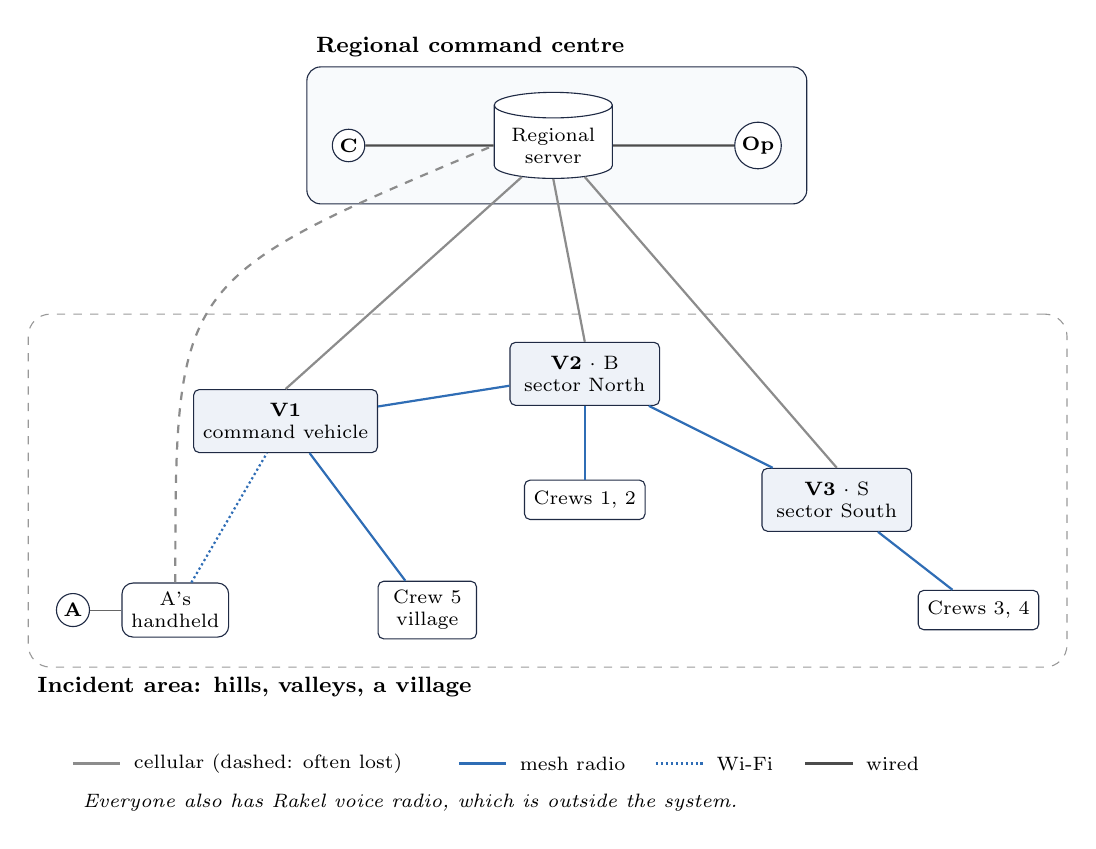
\begin{tikzpicture}[x=1cm,y=1cm, every node/.style={font=\scriptsize},
  veh/.style={draw=ink, fill=soft, rounded corners=2pt, minimum width=1.9cm,
              minimum height=.8cm, align=center},
  crew/.style={draw=ink, fill=white, rounded corners=2pt, minimum width=1.25cm,
               minimum height=.5cm, align=center},
  hh/.style={draw=ink, fill=white, rounded corners=4pt, minimum width=1.25cm,
             minimum height=.6cm, align=center},
  srv/.style={draw=ink, fill=white, cylinder, shape border rotate=90, aspect=.25,
              minimum width=1.5cm, minimum height=.9cm, align=center},
  person/.style={draw=ink, circle, fill=white, inner sep=1.3pt, font=\scriptsize\bfseries},
  cell/.style={draw=black!45, thick},
  mesh/.style={draw=accent, thick},
  wifi/.style={draw=accent, thick, densely dotted},
  wired/.style={draw=black!70, thick},
]
  % Regional command centre
  \node[srv] (srv) at (5,7.1) {Regional\\server};
  \node[person] (C) at (2.4,7.1) {C};
  \node[person] (O) at (7.6,7.1) {Op};
  \draw[wired] (C) -- (srv);
  \draw[wired] (O) -- (srv);
  \begin{scope}[on background layer]
    \node[draw=ink, fill=soft!40, rounded corners=5pt, fit=(srv)(C)(O), inner sep=9pt,
          label={[font=\footnotesize\bfseries, anchor=south west]north west:Regional command centre}] (cc) {};
  \end{scope}

  % Incident area
  \node[veh] (V1) at (1.6,3.6) {\textbf{V1}\\command vehicle};
  \node[veh] (V2) at (5.4,4.2) {\textbf{V2} $\cdot$ B\\sector North};
  \node[veh] (V3) at (8.6,2.6) {\textbf{V3} $\cdot$ S\\sector South};
  \node[crew] (K12) at (5.4,2.6) {Crews 1, 2};
  \node[crew] (K34) at (10.4,1.2) {Crews 3, 4};
  \node[crew] (K5) at (3.4,1.2) {Crew 5\\village};
  \node[hh] (HA) at (0.2,1.2) {A's\\handheld};
  \node[person] (A) at (-1.1,1.2) {A};
  \draw[black!60] (A) -- (HA);

  \begin{scope}[on background layer]
    \node[draw=black!40, dashed, rounded corners=8pt, fit=(V1)(V2)(V3)(K12)(K34)(K5)(HA)(A),
          inner sep=10pt, label={[font=\footnotesize\bfseries, anchor=north west]south west:Incident area: hills, valleys, a village}] (area) {};
  \end{scope}

  % Cellular backhaul (patchy)
  \draw[cell] (V1.north) -- (srv.south west);
  \draw[cell] (V2.north) -- (srv.south);
  \draw[cell] (V3.north) -- (srv.south east);
  \draw[cell, dashed] (HA.north) .. controls (0.2,5.4) .. (srv.west);
  % Mesh between vehicles and to crews
  \draw[mesh] (V1) -- (V2);
  \draw[mesh] (V2) -- (V3);
  \draw[mesh] (V2) -- (K12);
  \draw[mesh] (V3) -- (K34);
  \draw[mesh] (V1) -- (K5);
  % Wi-Fi between A's handheld and V1
  \draw[wifi] (HA) -- (V1);

  % Legend
  \begin{scope}[shift={(-1.1,-0.75)}]
    \draw[cell] (0,0) -- (.6,0); \node[anchor=west] at (.65,0) {cellular (dashed: often lost)};
    \draw[mesh] (4.9,0) -- (5.5,0); \node[anchor=west] at (5.55,0) {mesh radio};
    \draw[wifi] (7.4,0) -- (8,0); \node[anchor=west] at (8.05,0) {Wi-Fi};
    \draw[wired] (9.3,0) -- (9.9,0); \node[anchor=west] at (9.95,0) {wired};
  \end{scope}
  \node[anchor=west, font=\scriptsize\itshape] at (-1.1,-1.25)
    {Everyone also has Rakel voice radio, which is outside the system.};
\end{tikzpicture}
\caption{The setting. Every vehicle computer and handheld keeps a copy of the journal; the
regional server holds the most complete one. The incident commander A works from the
command vehicle V1 or from a handheld, whose cellular link is often lost in the valleys.}
\label{fig:setting}
\end{figure}

\section{The journal: entries, readers and statuses}
\label{sec:journal}

\textbf{Entries.} The journal holds three kinds of entry, each signed by the person who
made it:
\begin{itemize}
  \item \textit{Decisions}: orders, resource assignments, and decisions that intrude on
        property or rights. Only the person in command makes decisions.
  \item \textit{Field submissions}: observations, status reports and requests. Anyone may
        submit them; they need no authority and are never invalid.
  \item \textit{Authority records}: grants, succession rules, handovers, takeovers,
        activations and confirmations (\S\ref{sec:rules}). Only the person entitled to make
        each one can sign it.
\end{itemize}

\textbf{Readers.} People read the journal for different purposes and can accept different
delays (\cref{tab:readers}).

\begin{table}[htbp]
\centering
\caption{Who reads the journal, and what they need from it. To be checked with the
rescue service (\S\ref{sec:practice}).}
\label{tab:readers}
\small
\begin{tabularx}{\linewidth}{@{}P{2.6cm}P{3.9cm}P{3.5cm}L@{}}
\toprule
\textbf{Reader} & \textbf{Reads it to} & \textbf{Can work from entries that lag?} &
  \textbf{Must be able to see} \\
\midrule
Incident commander & Follow their own decisions and the incident picture & Own decisions
  are always local; other entries may lag & Which of their decisions others have received \\
A successor taking over & Continue where the previous commander stopped & No: needs every
  decision up to the change of command & Which decisions may still be missing \\
Sector leaders and crews & Receive orders and report & Yes, if the lag is visible & Who issued
  each order, under which authority, and its status \\
Operators & Follow the incident, dispatch, escalate & Yes, for minutes & How old the picture is,
  and what is not yet settled \\
Reviewers & Establish who decided what, under which authority & Any delay & The complete
  record, residual decisions included \\
\bottomrule
\end{tabularx}
\end{table}

\textbf{Statuses.} Each device gives every decision one of four statuses, computed from the
records it holds:
\begin{itemize}
  \item \sAuth: made by the person who held command at that time, and settled, so no record
        that could change this can still arrive;
  \item \sProv: valid on the records this device holds, but not yet settled;
  \item \sResid: made under a grant that had already been superseded. Kept, attributed and
        labelled for review; never merged and never dropped;
  \item \sDoubt: made so close to a change of command that clock error leaves the order
        open. A person decides.
\end{itemize}
A reader therefore sees not only what was decided, but how certain it is that it stands.

\section{What the organization decides, and what the system does}
\label{sec:split}

The system never decides who commands. It records and enforces what the organization has
decided, explicitly or by a rule agreed in advance. \Cref{tab:split} separates the two.

\begin{table}[htbp]
\centering
\caption{The organizational problems, which the system must not try to solve, and the
technical problems, which it must.}
\label{tab:split}
\small
\begin{tabularx}{\linewidth}{@{}LL@{}}
\toprule
\textbf{The organization decides (not technical)} & \textbf{The system does (technical)} \\
\midrule
Who commands, and who may take over & Records grants and succession acts, signed by the
  people entitled to make them \\
When command should move: doctrine, judgement, legal mandate & Applies the agreed rules the
  same way on every device \\
Whether a commander is fit to continue & Measures silence and applies the timeouts the
  organization chose \\
What to do about decisions made on the wrong side of a change & Keeps them, attributes them
  and labels them for review \\
How people who disagree settle it & Shows every reader who commands, as far as it knows, and
  how certain that is \\
Who is legally responsible & Keeps an attributable, tamper-evident record \\
\bottomrule
\end{tabularx}
\end{table}

Disagreement needs a sentence of its own. If two people both act as commander for a while,
crews can receive contradictory orders. No system can prevent that between people who
cannot reach each other. The policies in \S\ref{sec:policies} bound how long it can last,
and the journal makes every such decision visible afterwards.

\section{From org chart to system}
\label{sec:translation}

\Cref{tab:translation} translates each element of the command organization into the system.
Devices carry a person's rights but hold none of their own.

\begin{table}[htbp]
\centering
\caption{The translation from org chart to system.}
\label{tab:translation}
\small
\begin{tabularx}{\linewidth}{@{}P{5.6cm}L@{}}
\toprule
\textbf{In the organization} & \textbf{In the system} \\
\midrule
A person in a role & A principal with a personal credential \\
The right to command & That person's right to add decisions to the journal \\
Appointment by a superior & A role grant signed by the superior \\
A succession rule in doctrine & A rule signed in advance, at appointment, that every device
  applies \\
Succession of command & Reconfiguration of who may add decisions \\
One commander at a time & One writer of decisions at a time \\
The appointing officer & The configuration master, as in Vertical Paxos \\
Voice radio & A channel outside the system; its outcome is recorded as a signed act \\
The people who read the journal & A requirement per reader: how stale an entry it can accept \\
\bottomrule
\end{tabularx}
\end{table}

\textbf{Do we need consensus?} \Cref{tab:agreement} lists everything that has to be agreed,
who agrees it and when, and whether devices need consensus for it.

\begin{table}[htbp]
\centering
\caption{What has to be agreed, and whether devices need consensus for it.}
\label{tab:agreement}
\small
\begin{tabularx}{\linewidth}{@{}P{3.5cm}P{3.6cm}LP{2.4cm}@{}}
\toprule
\textbf{What must be agreed} & \textbf{Who agrees it, and when} & \textbf{What the system uses} &
  \textbf{Consensus between devices?} \\
\midrule
Who commands first & C, at appointment & A signed grant & No \\
Who may take over, on which trigger & The organization in advance; C signs it for this
  incident & A signed rule with timeouts $T$ and $T'$ & No \\
A planned handover & A and B, at the time, often by voice & A handover signed by A and
  accepted by B & No \\
A takeover by a superior & C, at the time & A takeover signed by C & No \\
Activation after silence & Nobody at the time: the rule decides & An activation signed by B,
  checked against the rule & No; needs bounded clock error \\
The order of one person's decisions & Nobody: a person signs one thing at a time &
  Per-person sequence number and GNSS time & No \\
Which side of a change a decision falls on & Nobody: the rule decides & The GNSS times of the
  decision and of the succession act & No; close calls are in doubt \\
Two conflicting succession acts & The org chart, in advance & Precedence: a superior's act
  outranks a subordinate's, and a person's later act outranks their earlier one & No \\
A decision two people share & The people involved, at the time & -- & Yes: out of scope \\
\bottomrule
\end{tabularx}
\end{table}

Our hypothesis follows from the table. While one person commands, the organization's prior
agreement (grants, rules and precedence) together with GNSS time replaces consensus between
devices. Every device classifies every decision with the same deterministic rule, so devices
that hold the same records reach the same verdict. What no rule removes is the trade-off in
\S\ref{sec:policies}. Consensus returns only where authority is shared, which is the plural
side of the thesis.

\section{The rules of the journal}
\label{sec:rules}

\textbf{Replication.} Every entry is a signed record. Devices keep every record they learn
of and pass it on over any link. Records are never changed, deleted or merged, so
duplicates and reordering do no harm: the records form a grow-only set.

\textbf{Who held command when.} Every device computes this from the authority records with
one rule: start from C's grant to A, apply the succession acts in time order, and resolve
conflicts by the precedence in \cref{tab:agreement}. An activation by B is valid only if B's
device had heard nothing from A's device, directly or through the regional server, for $T$.

\textbf{Status of a decision.} A decision by the person who held command at its time is
valid. One by a person whose grant had already been superseded is residual. One made within
the clock-error bound $\varepsilon$ of a change of command is in doubt. A valid decision stays
provisional until it is settled: once the regional server holds every authority record that
anyone entitled to change command could have signed before the decision (per-person
sequence numbers make that checkable), it signs a confirmation, and devices that receive it
mark the decision authoritative. The server decides nothing: it only confirms that the
records are complete.

\textbf{Enforcement when a decision is made.}
\begin{itemize}
  \item A device lets a person add a decision only if that person holds command according to
        the records on that device.
  \item Under S2 and S4, the commander's device stops accepting the commander's decisions
        when its lease runs out: after $L$ without contact with the regional server (S2), or
        after $T'$ without hearing from the deputy's device, directly or through the regional
        server (S4). A and B thus measure the same silence. The device shows the commander
        when, under the rule, command will pass.
  \item Field submissions are always accepted.
  \item A decision that arrives from another device is always kept. If it depends on an
        authority record this device has not yet received, it stays provisional until that
        record arrives.
\end{itemize}

\textbf{Assumptions.}
\begin{itemize}
  \item Messages may be delayed, duplicated and reordered, and are eventually resent.
  \item Devices have GNSS time, with clock error at most $\varepsilon$ while GNSS is available.
  \item Devices are not Byzantine, and credentials are not stolen.
  \item A person signs from one device at a time.
  \item The organization's rule is one commander at a time.
  \item Voice is outside the system; the system records only its outcome.
\end{itemize}

\textbf{Partition cases.}
\begin{itemize}
  \item \textbf{P-A}: only A's device is cut off.
  \item \textbf{P-B}: every vehicle loses its cellular link at once; the mesh at the scene still
        works.
  \item \textbf{P-C}: the mesh also splits, so A and B are in different parts.
\end{itemize}

\section{Succession policies}
\label{sec:policies}

While A is cut off, a design can provide at most two of three things: (a) A keeps
recording decisions; (b) command moves without A; (c) only one device accepts decisions.
Each policy in \cref{tab:policies} keeps two and gives up the third; the evaluation will
measure what each one costs. We take S3 as the anchor, because explicit transfer is what we
believe practice is. S4 is our proposal if the rescue service has nothing like it.

\begin{table}[htbp]
\centering
\caption{Succession policies while A is cut off. $L$ is a lease, $T$ the silence after which
a deputy may activate, and $T'$ the commander's own timeout. The entries are hypotheses to
test, not results.}
\label{tab:policies}
\footnotesize
\setlength{\tabcolsep}{3pt}
\begin{tabularx}{\linewidth}{@{}P{.5cm}P{2.6cm}P{2.1cm}P{2.1cm}P{1.45cm}P{1.75cm}P{1.75cm}L@{}}
\toprule
& \textbf{Policy} & \textbf{Trigger} & \textbf{Agreed by, and when} & \textbf{(a) A keeps
  recording} & \textbf{(b) Command moves without A} & \textbf{(c) One device accepts} &
  \textbf{Main cost} \\
\midrule
S0 & No succession during a partition & -- & The organization, in advance & Yes, without
  limit & Never & Yes & No command in the system if A is incapacitated \\
S1 & Immediate promotion through the regional server (what the prototype does) & An operator
  promotes B & The operator, at the time & For one lease $L$ & As soon as B reaches the
  server & No: overlap up to $L$ & Residual decisions; needs the server \\
S2 & Promotion after A's lease expires & An operator promotes B & The operator at the time;
  $L$ in advance & For $L$ & After $L$ plus a margin & Yes, if clock error is bounded &
  Takeover delayed by $L$ \\
S3 & Handover by A, or takeover by C & A hands over; or C decides, usually after trying
  voice & A and B, or C, at the time & Until A learns of it & When C's act reaches B & Only if
  A's device also has a timeout & Depends on C, and on the channel to A \\
S4 & Activation after silence & A silent for $T$ & The organization in advance; C signs it at
  appointment & For $T'$ & After $T$ & Yes, if $T - T'$ exceeds the message delay plus
  $\varepsilon$ & Short $T$ risks needless takeovers; long $T$ leaves no commander \\
S5 & Both record; reconcile later & -- & -- & Yes & Yes & No & The plural case: the edge of
  scope \\
\bottomrule
\end{tabularx}
\end{table}

\section{Storyboard}
\label{sec:storyboard}

Each step says what happens, who acts, on which device, over which link, and what readers
see. The steps follow the incident in time; \cref{fig:timeline} draws steps 4 to 7 under
S4 and under S3.

\begin{figure}[htbp]
\centering
\newcommand{\lanes}{%
  \foreach \y/\l in {3/A's handheld, 2/B (V2), 1/Regional server and C, 0/Crews}{
    \draw[black!25] (0,\y) -- (11.6,\y);
    \node[anchor=east, font=\scriptsize] at (-.1,\y) {\l};
  }
  \draw[->, black!55] (0,-.55) -- (11.8,-.55) node[right, font=\scriptsize]{time};
}
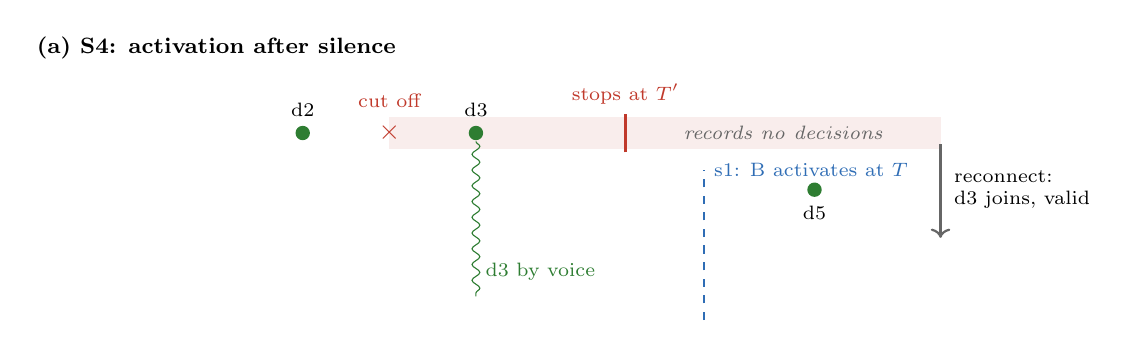
\begin{tikzpicture}[x=1cm, y=.72cm, every node/.style={font=\scriptsize}]
  \node[anchor=west, font=\footnotesize\bfseries] at (-2.6,4.5) {(a) S4: activation after silence};
  \lanes
  \fill[warn!9] (2,2.72) rectangle (9,3.28);
  \node[text=warn, font=\bfseries] at (2,3) {$\times$};
  \node[text=warn, above] at (2,3.28) {cut off};
  \fill[good] (.9,3) circle (2.6pt); \node[above] at (.9,3.12) {d2};
  \fill[good] (3.1,3) circle (2.6pt); \node[above] at (3.1,3.12) {d3};
  \draw[warn, line width=1.4pt] (5,2.66) -- (5,3.34);
  \node[text=warn, above] at (5,3.34) {stops at $T'$};
  \node[text=black!60, font=\scriptsize\itshape] at (7,3) {records no decisions};
  \draw[accent, dashed, thick] (6,-.3) -- (6,2.35);
  \node[text=accent, right] at (6,2.35) {s1: B activates at $T$};
  \fill[good] (7.4,2) circle (2.6pt); \node[below] at (7.4,1.88) {d5};
  \draw[good, decorate, decoration={snake, amplitude=.5mm, segment length=2mm}] (3.1,2.85) -- (3.1,0.12);
  \node[right, text=good] at (3.1,.55) {d3 by voice};
  \draw[->, black!60, thick] (9,2.8) -- (9,1.15);
  \node[right, align=left] at (9.05,2) {reconnect:\\d3 joins, valid};
\end{tikzpicture}

\vspace{6pt}
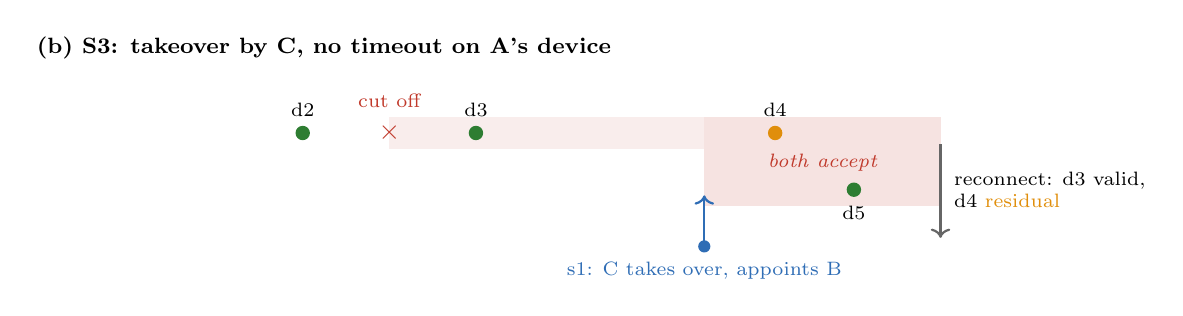
\begin{tikzpicture}[x=1cm, y=.72cm, every node/.style={font=\scriptsize}]
  \node[anchor=west, font=\footnotesize\bfseries] at (-2.6,4.5) {(b) S3: takeover by C, no timeout on A's device};
  \lanes
  \fill[warn!9] (2,2.72) rectangle (9,3.28);
  \fill[warn!14] (6,1.72) rectangle (9,3.28);
  \node[text=warn, font=\bfseries] at (2,3) {$\times$};
  \node[text=warn, above] at (2,3.28) {cut off};
  \node[text=warn, font=\scriptsize\itshape] at (7.5,2.47) {both accept};
  \fill[good] (.9,3) circle (2.6pt); \node[above] at (.9,3.12) {d2};
  \fill[good] (3.1,3) circle (2.6pt); \node[above] at (3.1,3.12) {d3};
  \fill[resid] (6.9,3) circle (2.6pt); \node[above] at (6.9,3.12) {d4};
  \fill[accent] (6,1) circle (2.2pt);
  \draw[->, accent, thick] (6,1.1) -- (6,1.9);
  \node[text=accent, below] at (6,.9) {s1: C takes over, appoints B};
  \fill[good] (7.9,2) circle (2.6pt); \node[below] at (7.9,1.88) {d5};
  \draw[->, black!60, thick] (9,2.8) -- (9,1.15);
  \node[right, align=left] at (9.05,2) {reconnect: d3 valid,\\d4 \textcolor{resid}{residual}};
\end{tikzpicture}

\vspace{3pt}
{\scriptsize \textcolor{good}{$\bullet$} valid (authoritative once settled)\quad
\textcolor{resid}{$\bullet$} residual\quad
\textcolor{accent}{\rule[.5ex]{1.2em}{1pt}} succession act\quad
\textcolor{warn}{$\times$} A's handheld is cut off}
\caption{Steps 4 to 7. Under S4 (a), A's handheld stops before B activates, so only one
device accepts decisions at a time, and A's valid decision d3 joins the journal when A
reconnects. Under S3 with no timeout on A's device (b), A and B both accept decisions after
C's takeover: A's order d4 to Crew~2 contradicts B's order d5, and d4 becomes residual.}
\label{fig:timeline}
\end{figure}

\begin{enumerate}[label=\textbf{\arabic*.}, leftmargin=1.6em]
  \item \textbf{Appointment.} C appoints A as incident commander and signs the succession
        rule for this incident: under S4, B is A's deputy with timeouts $T$ and $T'$; under
        S3 there is no rule, and command moves only by a handover from A or a takeover by C.
        Both records go from C's workstation to the regional server, and on to every device
        as it connects.
  \item \textbf{Normal operation.} From V1, A orders Crew~1 to hold the road in sector North
        (decision d1). d1
        reaches V2 over the mesh and the regional server over cellular. Crew~1 and the
        operators see d1 as \sProv, then as \sAuth\ when the server's confirmation arrives.
  \item \textbf{The commander moves.} A leaves V1 with a handheld to see the fire front from a
        ridge and, from the handheld, orders Crew~2 to the firebreak (d2) over cellular. Same
        person, another device: A's sequence number and GNSS time order d1 and d2. No change
        of command is involved, so timestamps are enough.
  \item \textbf{A is cut off (P-A).} In a valley, A's handheld loses cellular and is out of
        Wi-Fi and mesh range; voice still works. A orders Crew~2 back to the road (d3). d3
        stays on the handheld. Crew~2 hears it on the radio, but no other device can show
        it: a completeness gap, since d3 is valid but nobody else holds it yet. Under S4, A's
        handheld starts counting $T'$.
  \item \textbf{Cut off or incapacitated?} The network cannot tell, so people or the rule
        decide. Under S3, C calls A on Rakel. If A answers, nobody acts, and d3 reaches the
        journal later. If A does not answer, C signs a takeover appointing B (s1), which
        reaches V2 over cellular. Under S4, nobody acts: when B's device has heard nothing
        from A's for $T$, it offers B the activation, and B signs it (s1).
  \item \textbf{Overlap, or none.} Under S4, A's handheld stopped accepting A's decisions at
        $T'$, before B's activation, and showed A that under the rule B takes command at
        $T$. A passes what B needs by voice. Only B's device accepts decisions: B orders
        Crew~2 to the village edge (d5). Under S3 with no timeout, A's handheld still accepts
        A's decisions, and A sends Crew~2 to the north flank (d4). Crew~2 now holds two
        orders: A's by radio, and B's through its vehicle. This is the contradictory-orders
        case.
  \item \textbf{Reconnection.} A's handheld regains cellular. Records flow both ways, and
        every device applies the same rule. d3 was made before s1, so it is valid and the
        completeness gap closes. d4 was made after s1, so it is \sResid: kept, attributed to
        A, and shown to B and to the reviewers. A decision made within $\varepsilon$ of s1
        would be \sDoubt. A's handheld shows A that command passed to B at s1.
  \item \textbf{Escalation and a planned handover.} The fire grows and C comes to the scene.
        C signs a takeover from B. All links are up, so every device holds the takeover
        within seconds: no overlap and no residual decisions. Later, at a change of shift, C
        hands over to a relieving officer with a signed handover, which the officer accepts.
  \item \textbf{Everyone loses cellular (P-B).} A storm takes out the cellular network over
        the area; the mesh still works. Nothing reaches the regional server, so nothing is
        settled: every decision made from now on is \sProv. If A can still be reached over
        the mesh, A can hand over to B locally. If A falls silent, S4 lets B activate
        locally, because B's device can check the signed rule without the server. S1 and S2
        cannot move command, and under S3 C's takeover cannot reach the scene. When cellular
        returns, the server settles the decisions and its confirmations follow.
  \item \textbf{The mesh splits (P-C).} A and B end up in parts of the mesh that can reach
        neither each other nor the server. Under S4, A's device stops at $T'$ and B
        activates at $T$, so their devices never accept decisions at the same time. Under S3
        and S1, either command cannot move or both accept. When the parts rejoin, step~7
        applies.
\end{enumerate}

\section{Where each policy fails}
\label{sec:failures}

\begin{itemize}
  \item S4 fails if A's device ignores its timeout (a fault, or tampering), or if a link
        works in one direction only. A and B then both accept decisions, and A's decisions
        after s1 become residual.
  \item Every policy misclassifies decisions near a change of command if clock error exceeds
        $\varepsilon$. The in-doubt status contains the damage only while the bound holds.
  \item S3 cannot move command while C cannot reach the scene, and it overlaps if A's device
        has no timeout.
  \item S1 and S2 need the regional server, so they fail in P-B and P-C.
  \item Every policy fails with stolen credentials, which the model excludes. None covers
        shared authority, which needs agreement between people.
  \item Voice orders are outside the system under every policy. The journal can show who
        held command, but it cannot stop a person from giving orders by radio.
  \item No policy settles disagreement between people. The system shows it; the organization
        settles it.
\end{itemize}

\section{What we assume about practice}
\label{sec:practice}

We assume the following, and will check it with the rescue service:
\begin{itemize}
  \item The incident commander is the \textit{räddningsledare}, and the duty chief who appoints
        and may take over is the \textit{räddningschef i beredskap}.
  \item Command moves upward, by a takeover announced on Rakel; planned handovers happen at
        changes of shift.
  \item Activation of a deputy after silence is not current practice, so S4 is our proposal.
  \item Commanders sometimes lose data but keep voice.
  \item The devices and readers are as in \cref{tab:people,tab:readers}.
\end{itemize}

The questions we will ask:
\begin{enumerate}
  \item How is command handed over or taken over in practice, and how is it announced?
  \item Does anything like pre-authorized succession exist, for example a deputy taking over
        when the commander cannot be reached? Under what conditions?
  \item What would a reasonable $T$ be, in minutes, and who would decide it?
  \item Do commanders lose data but keep voice? How often, and for how long?
  \item Is command usually transferred upward, or to a designated deputy?
  \item Which devices do commanders, sector leaders and crews carry?
  \item Who reads the incident journal, during and after an incident, and for what?
\end{enumerate}

\section{Sign-off}
\label{sec:signoff}

Please confirm each item, or mark what should change:

\tick The incident, the people, devices and links (\S\S\ref{sec:incident}--\ref{sec:people})\\
\tick The journal's readers and the four statuses (\S\ref{sec:journal})\\
\tick The line between organization and system (\S\ref{sec:split})\\
\tick The translation, and the hypothesis that devices need no consensus while one person
commands (\S\ref{sec:translation})\\
\tick The rules of the journal and the assumptions (\S\ref{sec:rules})\\
\tick The policies, with S3 as the anchor and S4 as our proposal (\S\ref{sec:policies})\\
\tick The partition cases in scope: P-A, P-B and P-C (\S\ref{sec:rules})\\
\tick Whether the trade-off is argued, or model-checked for each policy

\end{document}
